\section{Background}
\label{sec:background}
%-------------------------------------------------------------------------------
In this section, we first present the workflow of the 3D face authentication system and then introduce the liveness detection in detail.

\subsection{3D Face Authentication}
Face authentication is a biological authentication scheme used to verify whether the user is legitimate. 3D face authentication system refers to such a system employing the 3D liveness detection module for its effectiveness and robustness in anti-spoofing. A standard  3D face authentication system works in three steps as shown in Figure.~\ref{fas_workflow}. When a user attempts to access a device or system with 3D face authentication, a visible light camera and an infrared camera are used to capture the RGB and depth images of the user simultaneously.

\textbf{Step 1: Face Detection.} 
The face detection step then detects and crops the face regions in the RGB and depth images. For RGB images, face detection algorithms such as multi-task convolutional neural network (MTCNN) \cite{zhang2016joint} are used to locate the face area in the RGB images and output the bounding-box coordinates. For depth images, the face area is determined by mapping the face bounding-box coordinates from RGB images.

\textbf{Step 2: Liveness Detection.} The liveness detection step analyzes the RGB and depth face images and extracts the 2D and 3D features to determine whether they belong to a live person. 
This step aims to defend against spoofing attacks such as printed photos, video replays, and masks~\cite{chakka2011competition,anjos2011counter,raghavendra2015presentation, bhattacharjee2018spoofing, nesli2013spoofing}.

\textbf{Step 3: Face Comparison.} Face images passing liveness detection are then fed into the face comparison step, which employs face comparison algorithms such as FaceNet~\cite{schroff2015facenet} to extract a feature vector from the input face image and calculate the distance between it and the pre-recorded feature vector in the database to verify if the user is the legitimate one.

From the workflow of the face authentication system, we find that the key to fooling 3D face authentication systems with a printed photo from a legitimate user is to bypass its liveness detection module.  In the following, we introduce the liveness detection in detail.

\begin{figure}[pt]
	\centerline{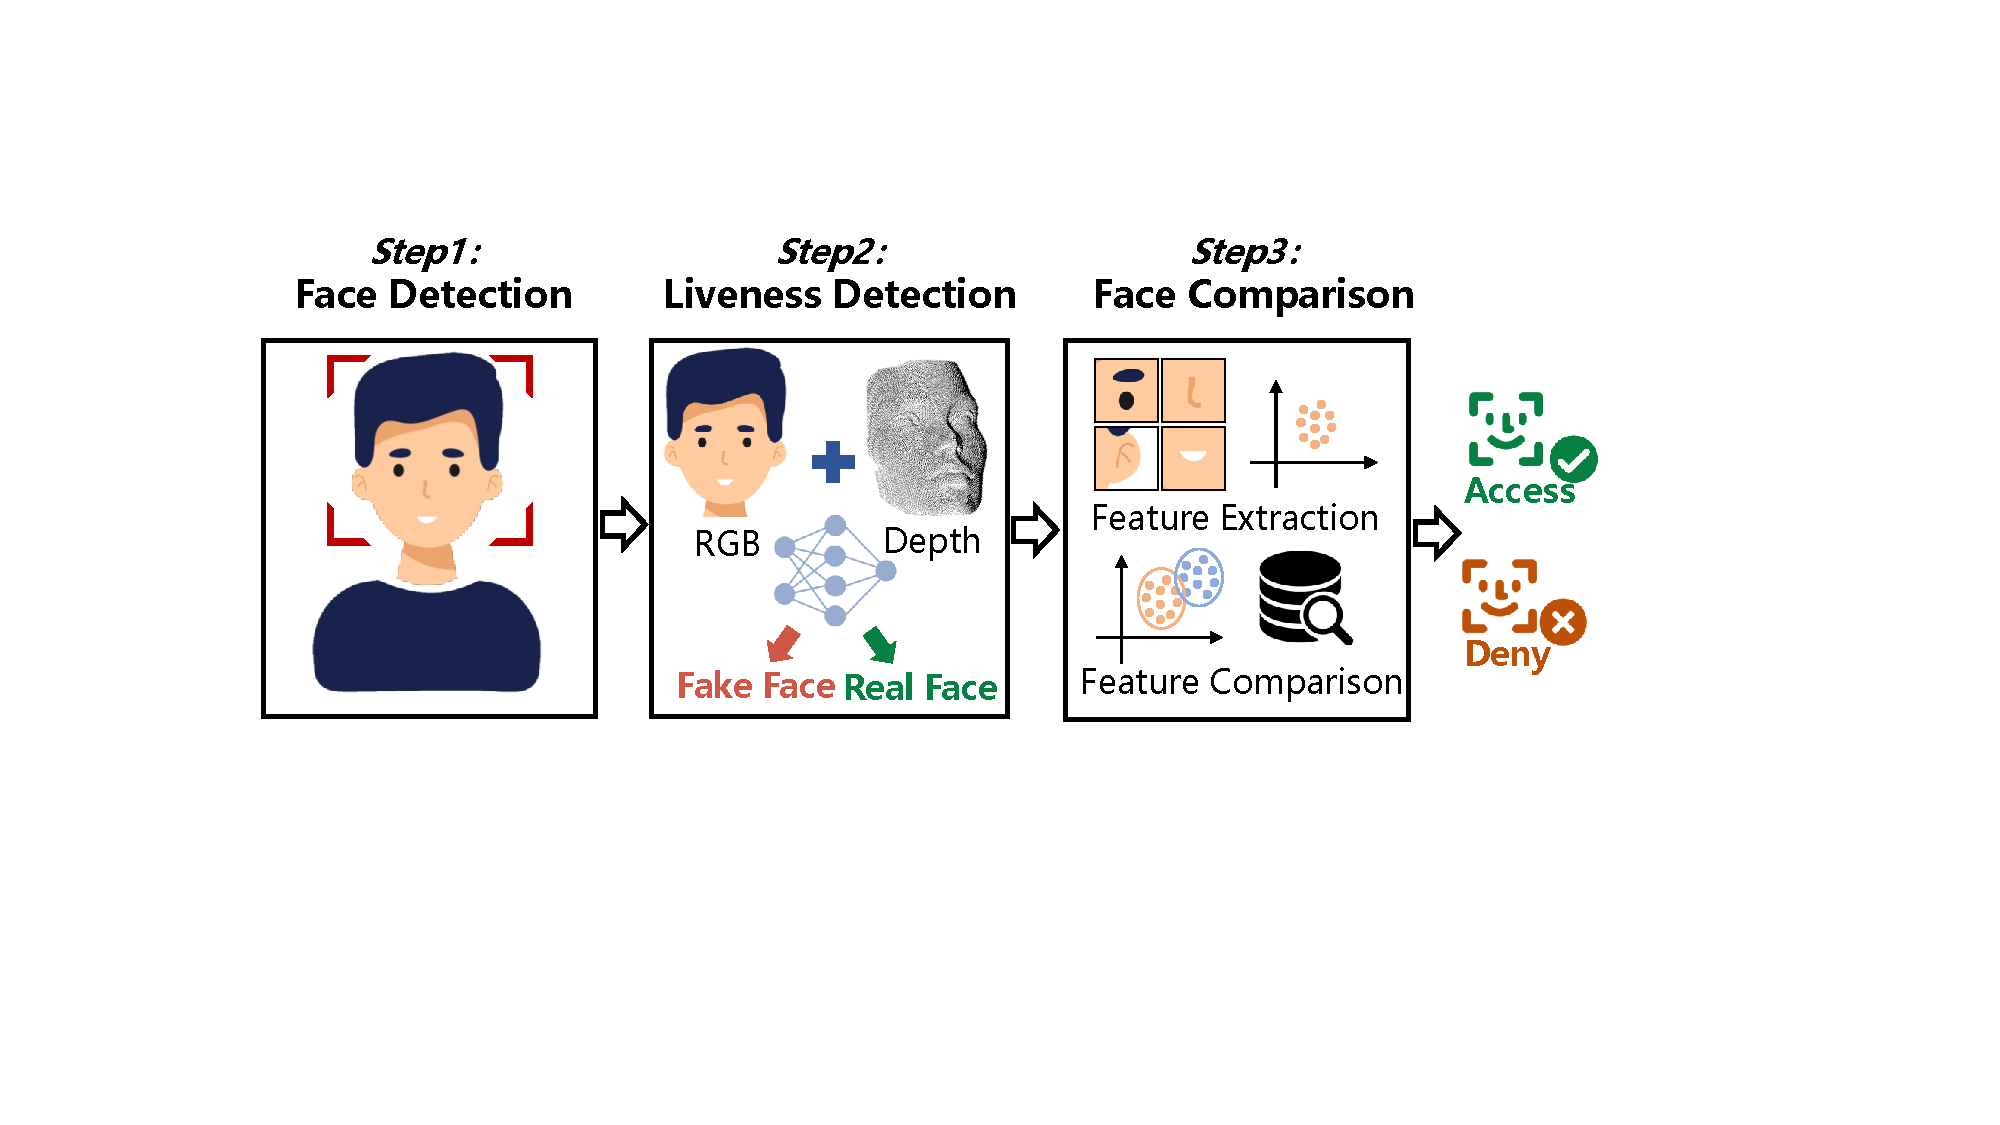
\includegraphics[width = 0.5\textwidth]{figures/face_auth_workflow.pdf}}
	\vspace{-0.15in}
	\caption{3D face authentication systems first detect faces on the captured RGB and depth images, then determine whether those faces are from real people, and finally verify whether they are from legitimate users. }
	\label{fas_workflow}
	\vspace{-0.15in}
\end{figure}

\subsection{Liveness Detection}
Liveness detection  determines
whether the captured face images belong to a live person. It aims to reject non-living objects with human traits presented to cameras that try to obfuscate the face authentication system. 
Existing liveness detection methods include two categories: (1) Active liveness detection that defines a certain action, e.g., blink or nod, and requires the user to perform it to determine whether the user is alive. This method is commonly used in cloud-service face authentication since they have less restriction on capturing sensors but require more computing resources. (2) Passive liveness detection that uses one-shot images to determine whether the user is alive. 
Since passive liveness detection is user-friendly and does not require user interaction, it is commonly used nowadays in smart locks, access control devices, etc~\cite{chakraborty2014overview}.  The 3D liveness detection we target is such a passive liveness detection method,  and we present the details of the 3D passive liveness detection in the following. 

\subsection{3D Passive Liveness Detection}

3D passive liveness detection utilizes both RGB and depth information to determine whether the user is alive.  The RGB images are captured by a visible camera. The depth images are obtained by depth cameras including (1) structured light cameras which use the infrared scatter pattern to encode depth information, (2) time-of-flight (ToF) cameras which calculate the depth by recording the infrared light echo time, and (3) stereo cameras which utilize binocular vision systems. Among them, because of the high resolution, insensitivity to visible light and low cost, the structured light depth camera is most common in face authentication systems such as FaceID~\cite{han2007face,bud2018facing}, Smartlock\cite{waseem2020face}, etc.

\begin{figure}[pt] 
	\centerline{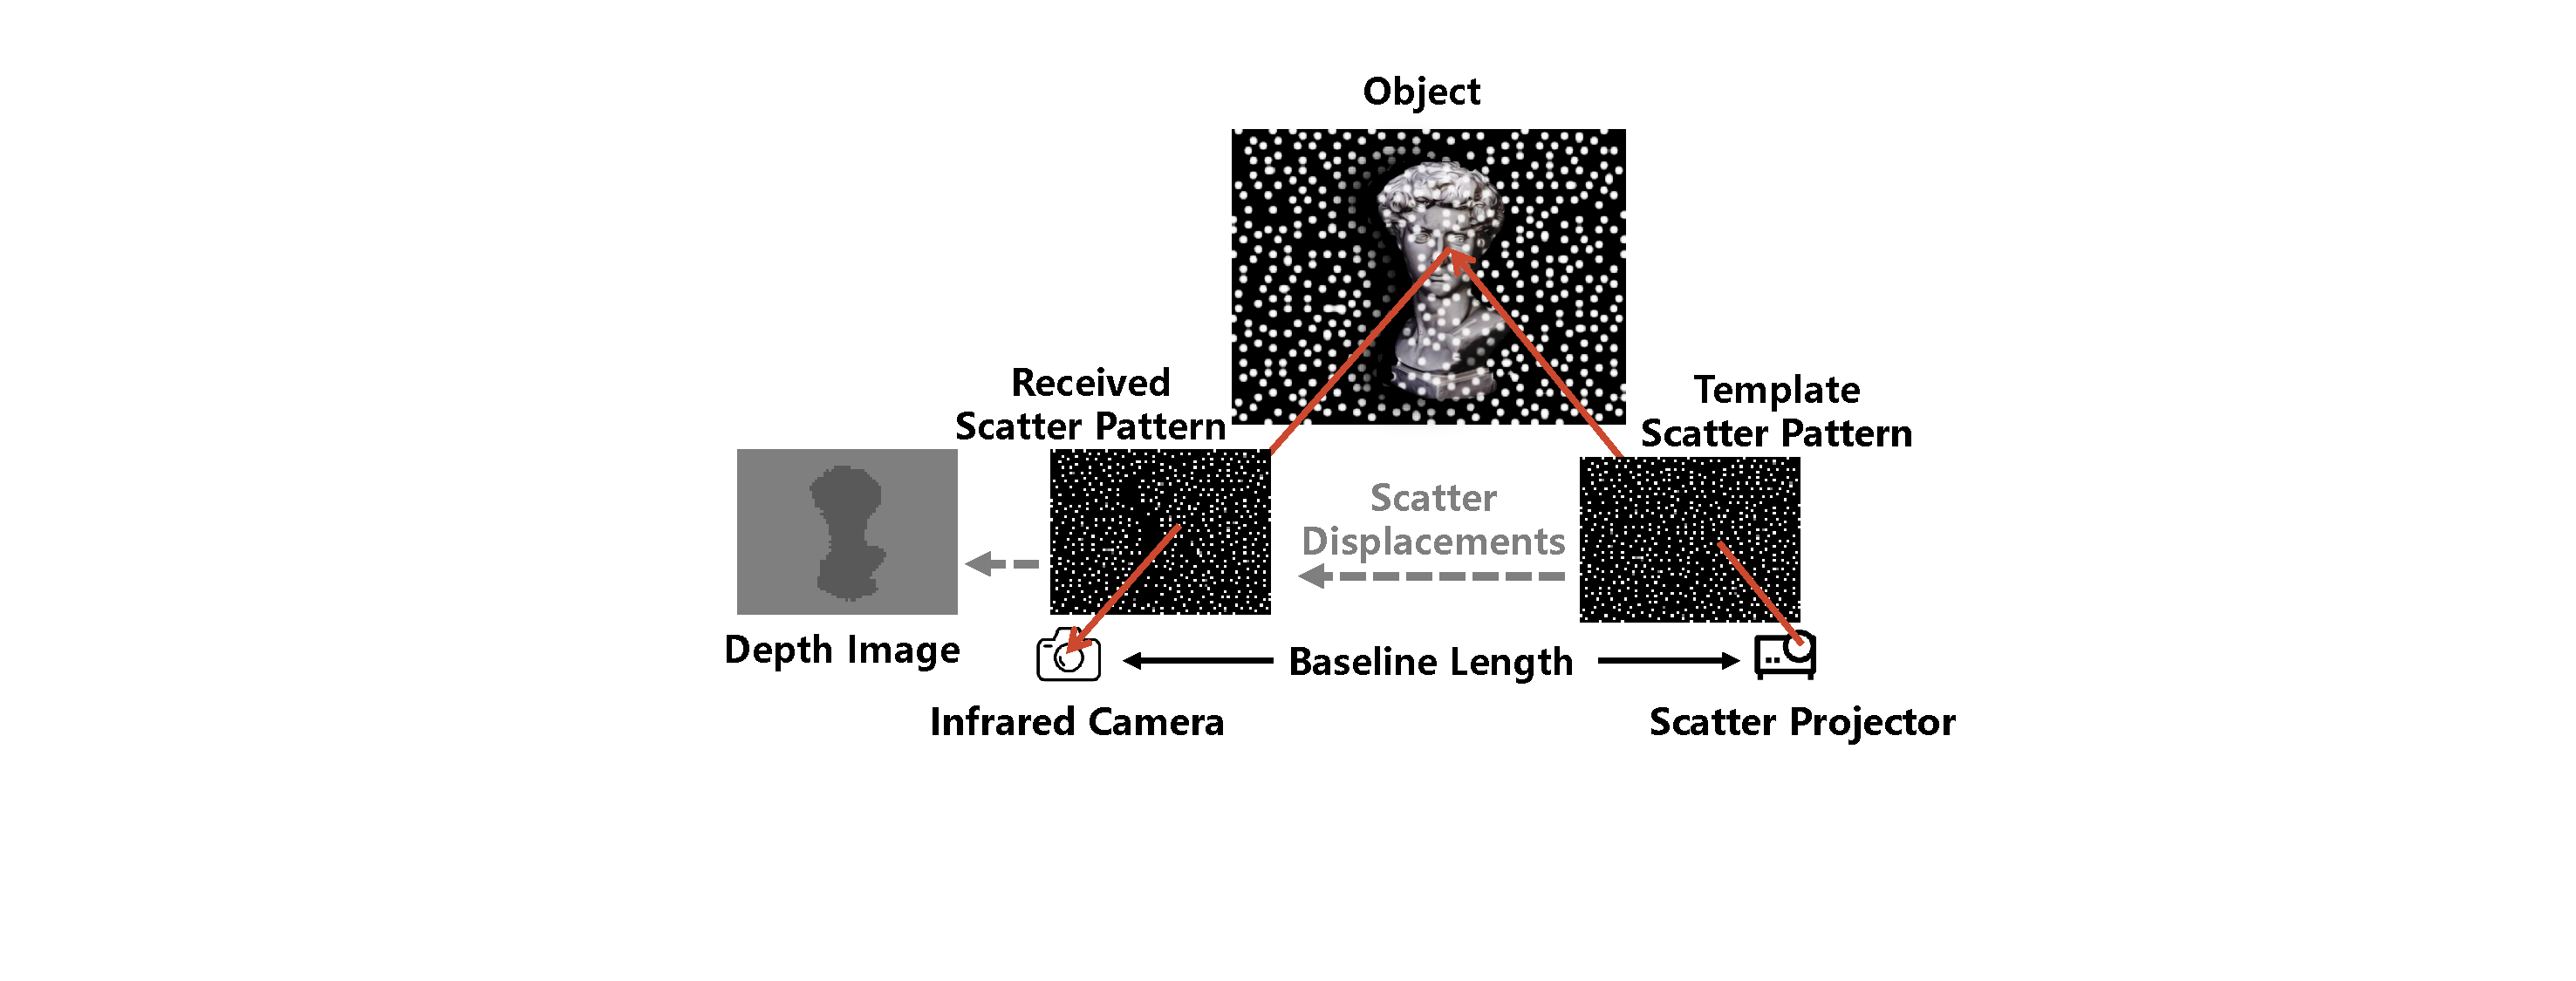
\includegraphics[width = 0.48\textwidth]{figures/structured_light_camera.pdf}}
	\vspace{-0.1in}
	\caption{The structured light depth camera actively projects a constant scatter pattern to the object, then captures the reflected scatter pattern and calculates the depth of the target by measuring its displacement from the template scatter pattern. }
	\label{depth_camera}
	\vspace{-0.15in}
\end{figure}

Due to its popularity, we analyze the structured-light-based 3D passive liveness detection module in this paper.
%A structured-light-based 3D passive liveness detection module (3D liveness detection module in short) consists of both hardware and software components.
%, where the former captures the face information of the user pending authentication while the latter processes the information and makes decisions.
%\textbf{Hardware.}
%The hardware component  of a 3D liveness detection module include a visible camera and a structured light depth camera, which capture the RGB and depth images of a legitimate user  simultaneously~\cite{zanuttigh2016time, daneshmand20183d}. 
A standard structured light depth camera contains a scatter projector and an infrared camera, as shown in Fig.~\ref{depth_camera}. The scatter projector can project a  constant infrared pattern containing tens of thousands of scatter points. The infrared camera can capture it at the reference depth plane and store it as a template scatter pattern. 
When capturing a depth image of the target, the reflected scatter pattern will be distorted due to the different depths. Then, the infrared camera will capture the distorted scatter pattern and calculate the depth information by measuring the displacement between each scatter point with the one in the template scatter pattern.

To illustrate how the structured light depth camera calculates the depth information from scatter displacements, we consider a single scatter point first.
% For simplicity, we take the depth calculation for a single scatter point as an example to illustrate how the structured light camera measures the depth from scatter displacements. 
As shown in Fig.~\ref{imaging_mechanism}, a scatter point $x_p$ reflected by the planes of  reference depth $d_{ref}$ and tatget depth $d_t$ are denoted as $x_{ref}$ and $x_{t}$ on the imaging plane of the infrared camera.
Based on the rule of the similar triangle, we can calculate $d_t$ as follows:
\begin{equation}
	d_t= \frac{d_{ref}Lf_c}{Lf_c - d_{ref}\Delta x_c}
	\label{d_cal}
\end{equation}
where $\Delta x_c=x_{ref}-x_{t}$ is the displacement between $x_{ref}$ and $x_{t}$. The baseline length $L$, the focal length $f_c$, and reference depth $d_{ref}$ are constant and known to the depth camera. In such a way, the camera can obtain the depth of a single point and even a complete face.

%Based on the similar triangles rule, we can calculate $x_{ref}$ and $x_{t}$ as follows:
%
%\begin{equation}
%	x_{ref}=\frac{f_c}{d_ref}(L-\frac{x_pd_ref}{f_p}) 
%	\label{xc1_cal}
%\end{equation}
%\begin{equation}
%	x_{t}=\frac{f_c}{d_t}(L-\frac{x_pd_t}{f_p}) 
%	\label{xc2_cal}
%\end{equation}
%where $f_c$ and $f_p$ are the focal length of the infrared camera and projector, and  $L$  is the baseline length (distance) between infrared camera and projector. 
%Based on them, we can calculate ${d_t}$ as follows:
%\begin{equation}
%	%\frac{1}{d_1} - \frac{1}{d_2} = \frac{\Delta x}{Lf_c} 
%	d_t= \frac{d_refLf_c}{Lf_c - d_ref\Delta x_c}
%	\label{d_cal}
%\end{equation}
%where $\Delta x_c=x_{ref}-x_{t}$ is the displacement between $x_{ref}$ and $x_{t}$. The baseline length $L$, the focal length $f_c$, and reference depth $d_ref$ are constant and known to the depth camera. In such way, the camera can obtain the depth of a single point and even a complete face.


\begin{figure}[!t]
	\centering
	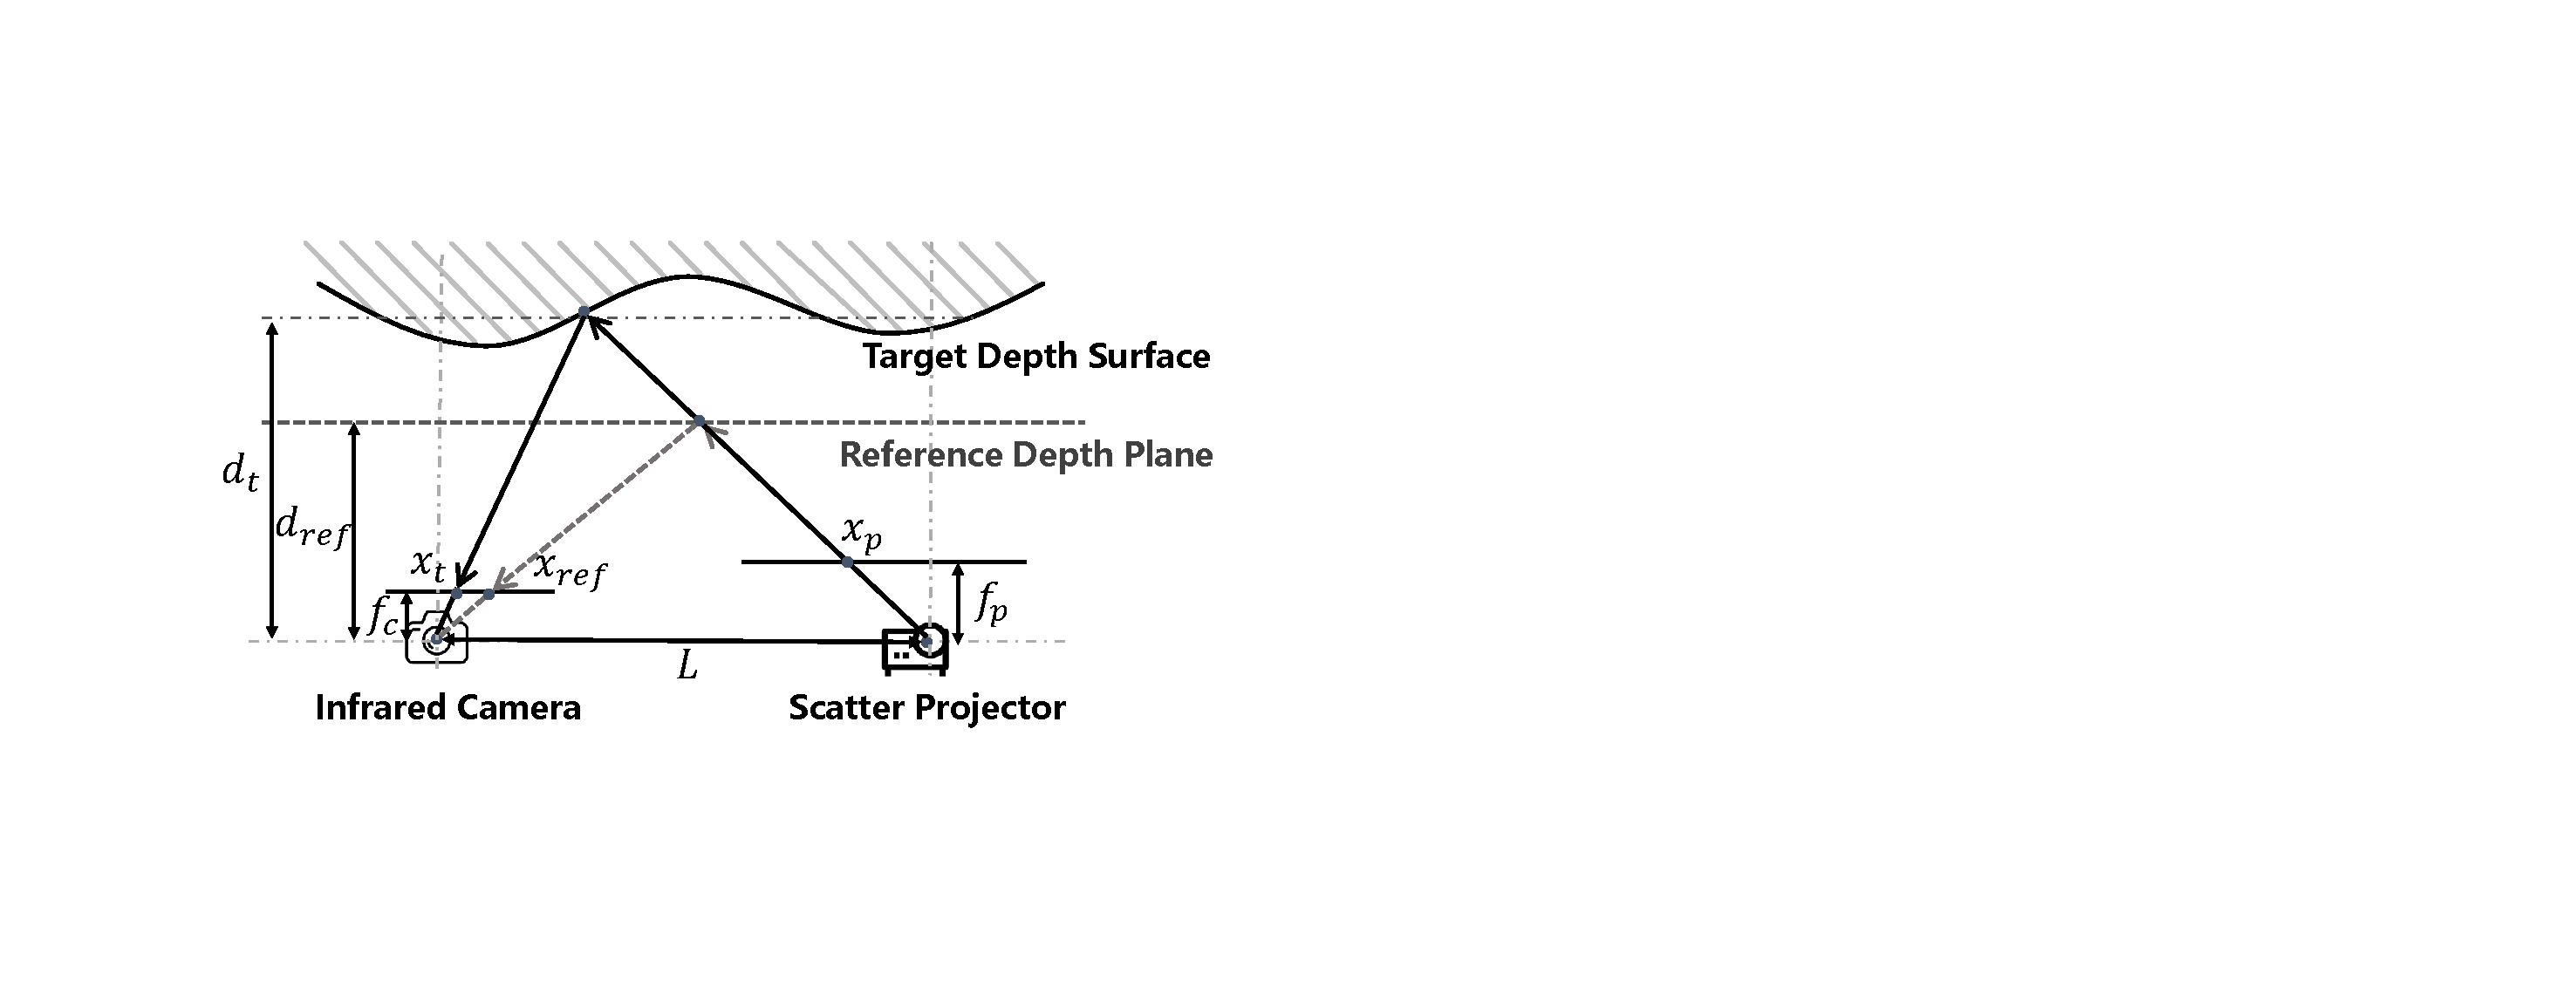
\includegraphics[width=0.48\textwidth]{figures/imaging_mechanism.pdf} 
	\vspace{-0.1in}
	\caption{Imaging mechanism of the structured light camera. The scatter projector projects the scatter point to the reference depth plane and the target depth, then the infrared camera captures the reflected scatter points and calculates the target depth by measuring the displacement between them. }
	\label{imaging_mechanism}
	\vspace{-0.15in}
\end{figure}

After obtaining RGB and depth images, the 3D liveness detection module utilizes both of them for decisions.
For RGB images, it uses deep learning algorithms, e.g., Convolution Neural Networks (CNNs)~\cite{yang2014learn, chen2020face, luo2018face} or Vision Transformer (Vit)~\cite{george2020effectiveness}, to extract features such as edges, textures, Moiré patterns or features in the frequency domain,  and then utilizes a binary classifier to determine them as true or fake faces with confidence scores.
For depth images, it first maps it to the RGB image and locates the face region. Then, it uses feature point matching~\cite{goswami2014rgb} or CNNs~\cite{george2021cross, te2020exploring} to determine whether the face belongs to a real person by detecting the special geometric structure of the human face. 

%\textbf{Hardware.} The
%3D liveness detection module uses a visible camera to capture the RGB image of a legitimate user and a structured-light depth camera~\cite{zanuttigh2016time, daneshmand20183d} to capture the depth image at the same time. 
%A standard structured-light depth camera contains a scatter projector and an infrared camera, as shown in Fig.~\ref{depth_camera}.
%During capturing depth images,  the projector first projects a fixed infrared scatter pattern to the target, which will suffer from different deformations due to the different depths of the target. Then, the infrared camera will capture the reflected scatter pattern from the object and compare it with the projected scatter pattern.  By measuring the displacement of each scatter with the disparity estimation algorithm~\cite{fanello2016hyperdepth}, it calculates the depth of the target.

%\textbf{Software.} After obtaining RGB and depth images at the same time, 3D liveness detection module utilizes both of them for decisions.
%For RGB images, it uses deep learning algorithms, e.g., Convolution Neural Networks (CNNs)~\cite{yang2014learn, chen2020face, luo2018face} or Vision Transformer (ViT)~\cite{george2020effectiveness}, to extract features such as edges, textures, moiré patterns or features in the frequency domain,  and then utilizes a binary classifier to determine them as true or fake faces with confidence scores.
%For depth images, it first maps it with the RGB image and locates the region of the face. Then, it uses feature point matching~\cite{goswami2014rgb} or CNNs~\cite{george2021cross, te2020exploring} to determine whether the face belongs to a real person by detecting the special geometric structure of the human face. 




%\textbf{Hardware. }
%3D passive liveness detection uses a visible camera to capture the RGB image of a legitimate user and a structured-light depth camera~\cite{zanuttigh2016time, daneshmand20183d} to capture the depth image at the same time. 
%A standard structured-light depth camera contains a scatter projector and an infrared camera, as shown in Fig.~\ref{depth_camera}.
%During capturing depth images,  the projector first projects a fixed infrared scatter pattern to the target, which will suffer from different deformations due to the different depths of the target. Then, the infrared camera will capture the reflected scatter pattern from the object and compare it with the projected scatter pattern.  By measuring the displacement of each scatter with the disparity estimation algorithm~\cite{fanello2016hyperdepth}, it calculates the depth of the target.
%
%\textbf{Software. } After obtaining RGB and depth images at the same time, 3D liveness detection utilizes both of them for decisions.
%For RGB images, it uses deep learning algorithms, e.g., Convolution Neural Networks (CNNs)~\cite{yang2014learn, chen2020face, luo2018face} or Vision Transformer (ViT)~\cite{george2020effectiveness}, to extract features such as edges, textures, moiré patterns or features in the frequency domain,  and then utilizes a binary classifier to determine them as true or fake faces with confidence scores.
%For depth images, it first maps it with the RGB image and locates the region of the face. Then, it uses feature point matching~\cite{goswami2014rgb} or CNNs~\cite{george2021cross, te2020exploring} to determine whether the face belongs to a real person by detecting the special geometric structure of the human face. 

%(2) IR-based liveness detection, which actively projects infrared light to target object and identifies the real face through comparing the difference of reflection features between the real human face and other spoofing materials. 
%(3) RGB+IR liveness detection, which combines the advantages of RGB-based and IR-based liveness detection and can work in different lighting conditions. 
%3D passive liveness detection is RGB-Depth-based (RGBD-based in short), which uses the depth information as an auxiliary feature in anti-spoofing. The algorithm reconstructs a 3D structure from depth image and uses it to determine whether the target is a real person or not.

%\subsection{Spoofing Attacks against Face Authentication}
%
%Existing spoofing attacks against face authentication mainly focus on the face comparison step, i.e., approximating the feature vector of a legitimate user in the face feature representation space. In this area, much work~\cite{sharif2016accessorize, singh2022powerful, nguyen2020adversarial, guo2021meaningful, komkov2021advhat, zolfi2021adversarial} has demonstrated the feasibility of fooling deep-learning-based face comparison algorithms with adversarial examples, which can render the algorithms identify an adversary as a legitimate user.However, those attacks mainly work for RGB images and may lose their attack capabilities when depth features are used \cite{belli2022personalized}.  
%Another aspect of spoofing face authentication is to deceive its 3D liveness detection. Existing work to achieve it is using an ultra-realistic 3D face mask~\cite{bhattacharjee2018spoofing}, but it requires a detailed 3D modeling of the victim and a high cost (over $\$4,000$). In this paper, we investigate the possibility of fooling face authentication with a low-cost printed photo.





%Face spoofing attacks use artifacts to spoof liveness detection systems. The most common way is the replay attack. The current replay attacks usually use high-precision printer to print the photo or high-resolution monitor to replay the video of the victim. Additionally, there are attackers who design ultra-realistic face mask to spoof liveness detection. However, the multi-modal liveness detection can prevent these attacks by identifying the specific texture or optical features.  
%
%There are other face spoofing attacks are emerging nowadays which taking over the camera feed and injecting the pre-designed image or video. Deepfake attack is one of the injecting attack, which uses synthetic face data and injects it into the camera. However, injecting attacks are all need intrusion into the hardware or software of liveness detection systems and are difficult to deploy in the real world.
%
%Therefore, in this paper, we conduct replay attacks which are more easier to deploy in the real world and propose different replay attacks for different modalities to against multi-modal liveness detection systems.